\subsection{計測系}
データロガーには、植松電機殿所有のEDX-100Aを用いた。サンプリングレートは200Hzとした。計測項目を以下に示す。
\begin{description}
\item[P1]GHe供給圧
\item[P2]オリフィス差圧
\item[P3]インジェクタ上流圧
\item[P4]プリバーナ圧
\item[P5]混合室圧
\item[Q1]LOX体積流量
\item[T1]オリフィス下流温度
\item[T2]インジェクタ上流温度
\item[T3]ノズル上流温度(内径)
\item[T4]ノズル上流温度(中心)
\item[T5]ノズル下流温度
\item[T6]予鈴温度
\item[T7]インジェクタフランジ温度
\end{description}
供試体周りの計測系の概略図を図\ref{}に、ノズル付近の内観を図\ref{fig:NozzleThermo}示す。
\\
高速度カメラによる可視化データ取得も行った。

\begin{figure}[htbp]
\begin{tabular}{cc}
\begin{minipage}{.5\textwidth}
\begin{center}
\centering
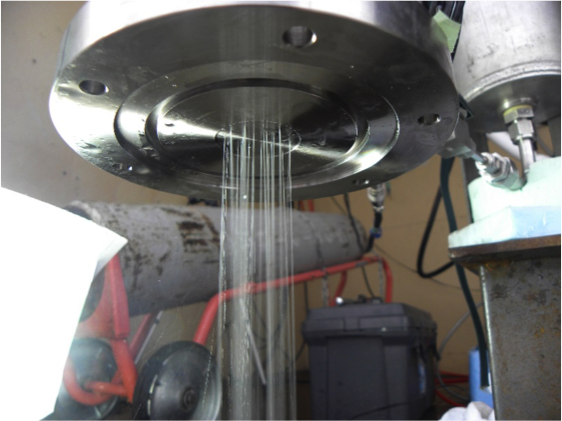
\includegraphics[width=7cm]{\FigAddTwo/Injector.png}
\caption{インジェクタ外観}
\label{fig:Injector}
\end{center}
\end{minipage}
\begin{minipage}{.5\textwidth}
\begin{center}
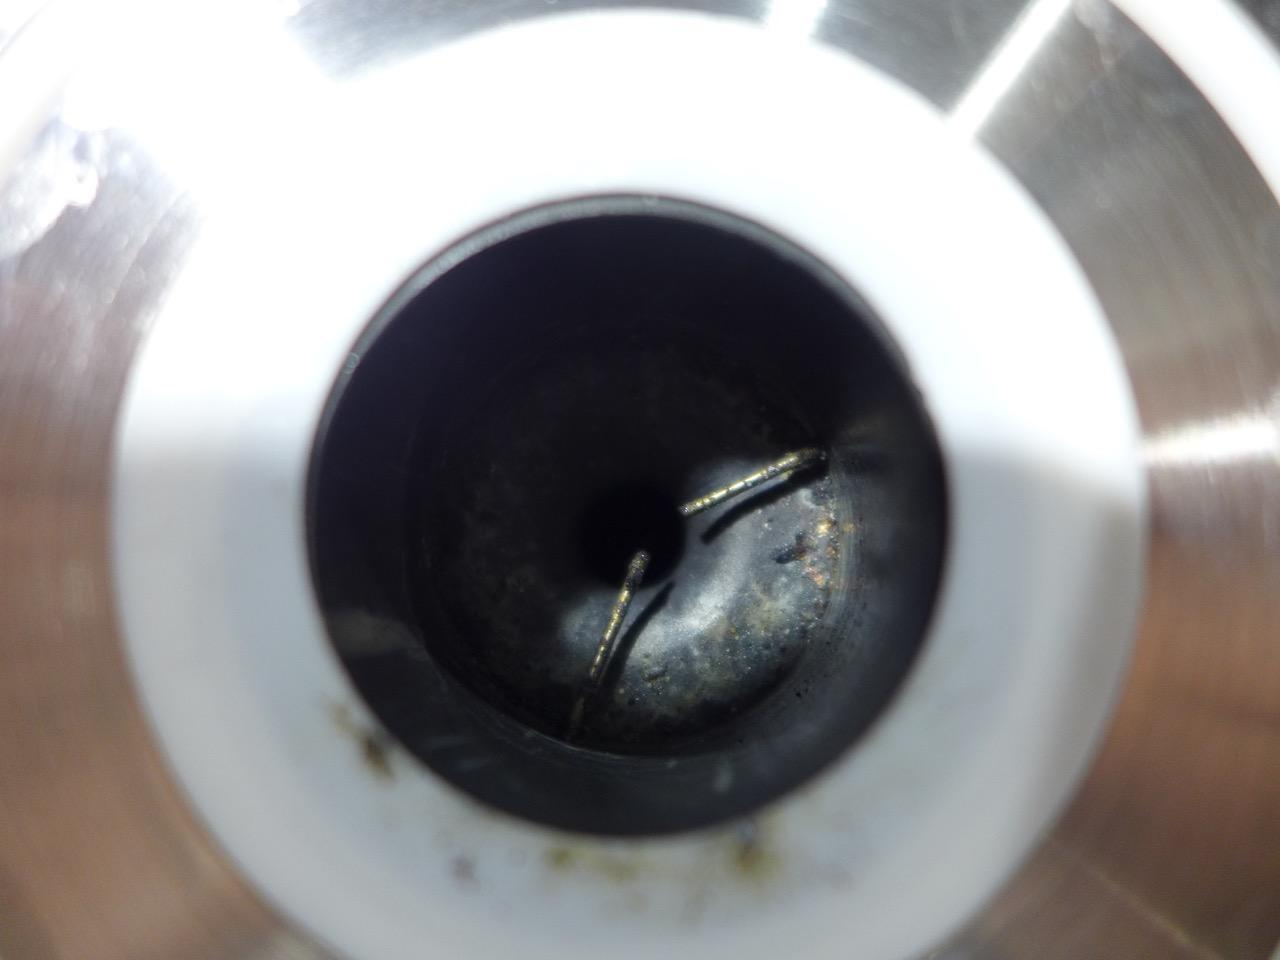
\includegraphics[width=7cm]{\FigAddTwo/NozzleThermo.jpg}
\caption{ノズル付近内観}
\label{fig:NozzleThermo}
\end{center}
\end{minipage}
\end{tabular}
\end{figure}
